\subsubsection{WAVE}
% 
\begin{center}
\textquote[\cite{VehicularTechnologySociety2014IEEEArchitecture}]{\emph{WAVE protocols are designed to allow applications to exchange data in a consistent, interoperable, and timely manner.}}
\end{center}\par
% 
Wireless Access in Vehicular Environments (WAVE) is a set comprising multiple standards, that aims for enabling V2V and V2I connectivity. Group of WAVE standards includes extensions to the MAC layer of 802.11 and several standards from the 1609 family. These standards specify the means of wireless communication on the four OSI model layers (physical, data link, network and transport layer). Furthermore, two standards specify the 'vertical' properties of the communication, such as security and remote management. Figure \ref{fig:wave-fam} shows part of the WAVE set in detail, while Table \ref{tab:wave-stds} lists WAVE standards and their use. The WAVE family specifies certain frequency allocations and channels for the use in the US. While the frequencies could be adjusted for the use in other countries, standard bodies in Europe have developed own standard, thus we will skip certain details of how WAVE works. Europan ITS-G5 is discussed \hyperref[sec:ITS-G5]{in the following section}.\par
% 
\begin{figure}
    \centering
    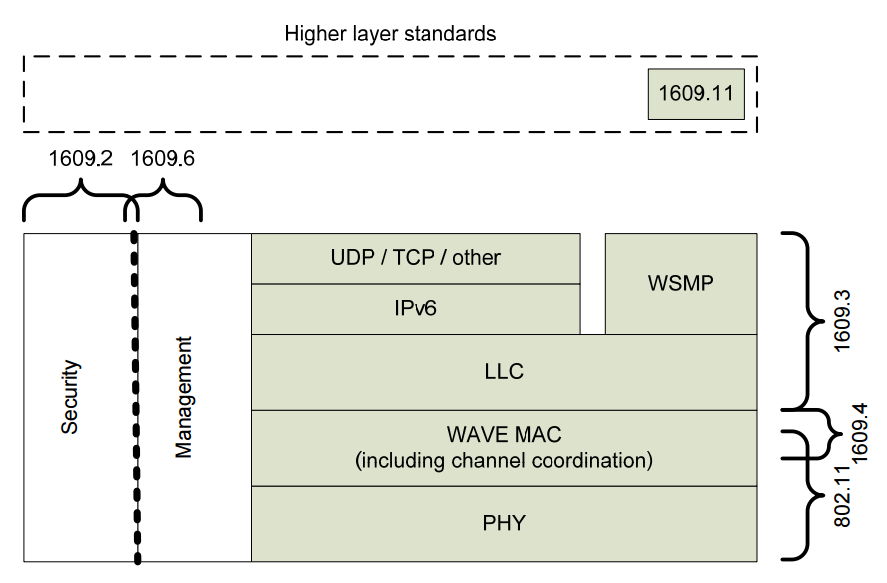
\includegraphics[width=.95\textwidth]{wave-fam}
    \caption{The standards of the WAVE set shown together with the elements of the OSI model. Taken from \cite{VehicularTechnologySociety2014IEEEArchitecture}}
    \label{fig:wave-fam}
\end{figure}

\begin{sidewaystable}
    \centering
    \begin{tabular}{|p{5cm}|p{5cm}|p{9cm}|}
        \hline
         \textbf{IEEE Standard} & \textbf{Area} & \textbf{Features} \\
         \hline
         IEEE Std 1609.4-2010 & Extensions to IEEE 802.11 MAC layer. & 
         \begin{itemize}[nolistsep,noitemsep, topsep=0pt]
             \item Channel timing
             \item MAC addressing \& pseudo-anonymity
         \end{itemize} \\ \hline
        %  
         IEEE Std 1609.3-2010 & Networking Services & 
         \begin{itemize}[nolistsep,noitemsep, topsep=0pt]
             \item WAVE service advertisement and channel scheduling
             \item WAVE Short message protocol
         \end{itemize} \\ \hline
        %  
         IEEE Std 1609.2-2013 & Security Services for Applications and Management Messages &
         \begin{itemize}[nolistsep,noitemsep, topsep=0pt]
             \item Security for WAVE Service Advertisements and WAVE Short Messages
             \item Additional security services
         \end{itemize} \\ \hline
        %  
        IEEE Std 1609.11-2010 & Over-the-Air Electronic Payment Data Exchange Protocol for ITS & ISO-compliant payment protocol \\ \hline \hline
        %  
        \textbf{IEEE Project} & \textbf{Area} & \textbf{Features} \\ \hline
        % 
        IEEE P1609.6  & Remote Management Services & Over the air management and aliasing. \\ \hline
        % 
        IEEE P1609.5  & Communication Manager & Network management \\ \hline
    \end{tabular}
    \caption{Set of WAVE standards and their respective areas. From \cite{VehicularTechnologySociety2014IEEEArchitecture}}.
    \label{tab:wave-stds}
\end{sidewaystable}
% 
As specified in \cite{VehicularTechnologySociety2014IEEEArchitecture}, WAVE standards do not distinguish between types of devices connected. Instead, they are robust enough to accommodate communication to/from On-board Units (OBU), Road-side Units (RSU), together with portable units (e.g. smartphones) and pedestrian units (e.g. roadside workers). 
% 
\subsubsection*{Extensions of 802.11 MAC layer} 
The 802.11 standard and in particular its amendment 802.11p can be seen as the roots for the WAVE family. 802.11p specifies the PHY and MAC layers of wireless communication suitable for vehicular environments. The newest revision of 1609.4 standard - IEEE Std 1609.4-2016 specifies some additional features of the MAC layer. It operates on frequency band 5.850GHz to 5.925GHz. While 0.005GHz at the lower edge is kept in reserve, the rest of the band is divided into 7 channels. These are further divided into Control Channel (CCH) and Service Channels (SCH). Figure \ref{fig:wave-channels} describes channel allocation in detail.\par
% 
\begin{figure}[ht]
    \centering
    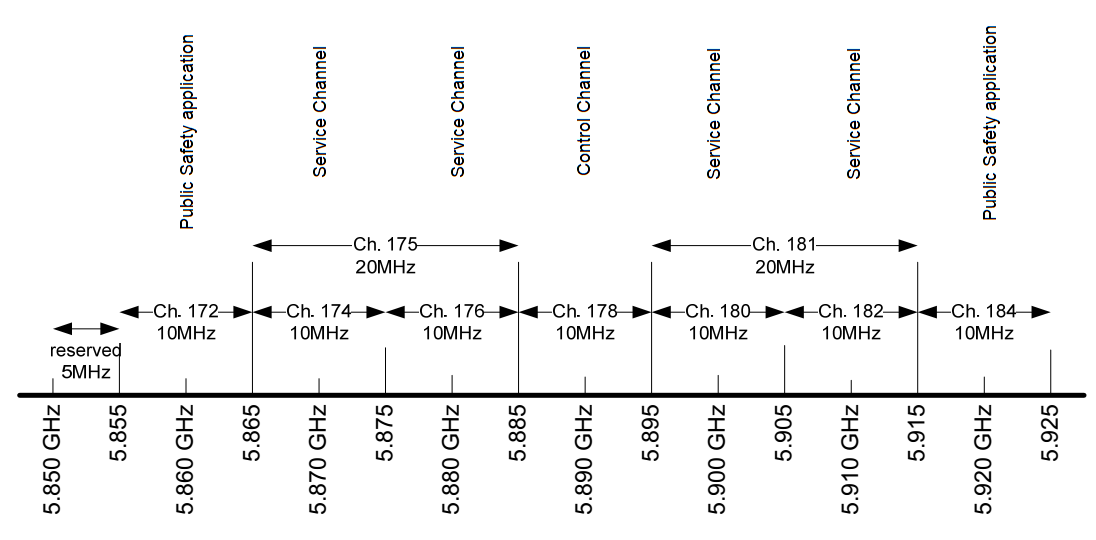
\includegraphics[width=.95\textwidth]{wave-channels}
    \caption{Figure showing channel frequencies and the use of the channels. Note that channels 174 and 176 and channels 180 and 182 can be merged to create channels 175 and 181 respectively. Taken from \cite[p. 20]{VehicularTechnologySociety2014IEEEArchitecture} (edited).}
    \label{fig:wave-channels}
\end{figure}
% 
The CCH is reserved for system management messages and only allows communication via WAVE Short Message protocol (WSMP). On SCH, both IP traffic (using IPv6 addresses) and WSMP is possible. WSMP is a protocol that sends WAVE Short Messages (WSM), which are designed to consume minimal channel capacity. WSMP allows transmitter device to specify physical characteristics of the transmission, such as transmitter power and channel used. The transmitter needs to provide MAC address of the receiver, however group MAC addresses are allowed. Furthermore, transmitter needs to provide a Provider Service Identifier (PSID)\footnotemark. The receiver can decide, based on the PSID of received WSM, if the message is of interest or should be discarded.
% 
\footnotetext{\textquote[\cite{20161609.12-2016Allocations}]{PSID is an integer with a value from 0 to 270 549 119. [...] Each allocated PSID value is associated with an organisation that is authorised to describe the use of that PSID.}}